\documentclass[10pt]{article}
\usepackage{amsmath}
\usepackage{listings}
\usepackage{graphicx}
\usepackage{amsmath}
\usepackage[margin=0.5in]{geometry}
\graphicspath{ {./images/} }
\begin{document}
{\centering
    CS7CS4 Machine Learning - Week 2
    \par
    Arnav Bhattacharya - 22307812
    \par
    Dataset \# id:6--6--6 
    \par
}
\section*{Question a}
Appendix contains all code for all questions and their respective subparts.

\subsection*{Part i}

\textbf{Visualise the data you downloaded by placing a marker on a 2D plot for each pair of feature values i.e. for each row in the data. On the plot the x-axis should be the value of the first feature, the y-axis the value of the second feature and the marker should be, for example, a '+' marker when the target value is +1 and a 'o' when the target is {\textendash}1. Your plot should look similar in style to this (with different data points of course!) Be sure to include a legend explaining what markers/colours are used for the +1 and -1 points.}

\vspace{5mm}
\begin{center}
  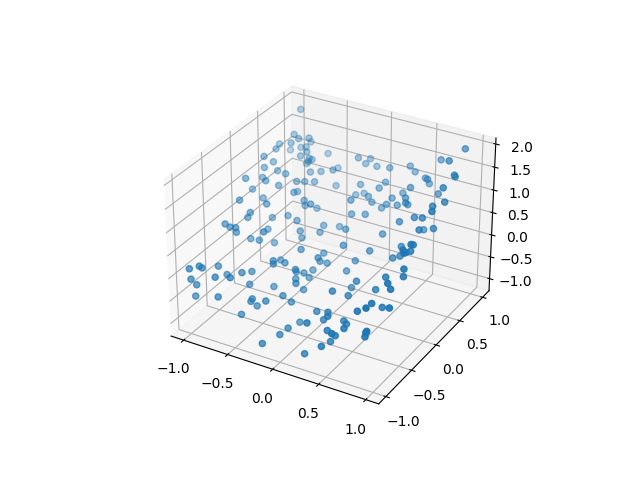
\includegraphics[scale=0.4]{Figure_1.png}
\end{center}

\subsection*{Part ii}
\textbf{Use sklearn to train a logistic regression classifier on the data. Give the logistic
regression model for predictions and report the parameter values of the trained
model. Discuss e.g. which feature has most infliuence on the prediction, which
features cause the prediction to increase and which to decrease.}

\begin{equation*}
    \theta_{0} + \theta_{1}x_{1} + \theta_{2}x_{2} = 1.81954024 - 0.25638908x_{1} + 4.80424731x_{2}
\end{equation*}
\vspace{1mm}

\begin{center}
  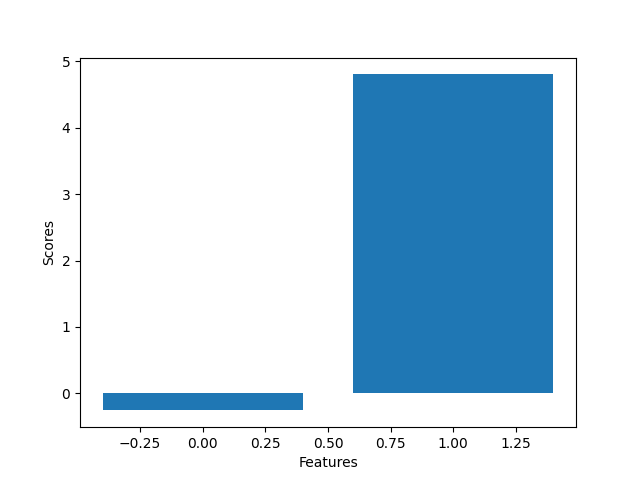
\includegraphics[scale=0.4]{Figure_2.png}
\end{center}

Using feature selection(the plot above), I found that the second feature(X2) has more impact on the predicted value.


\subsection*{Part iii}
\textbf{Now use the trained logistic regression classifier to predict the target values
in the training data. Add these predictions to the 2D plot you generated in
part (i), using a different marker and colour so that the training data and the
predictions can be distinguished. Show the decision boundary of the logistic
regression classifier as a line on the plot (you’ll need to use the parameter values
of the trained model to figure out what line this should be - explain how you
obtain it).}
\vspace{1mm}

\begin{center}
  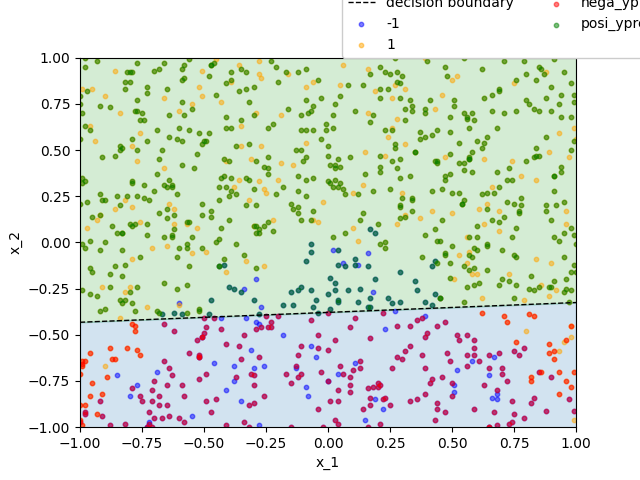
\includegraphics[scale=0.4]{Figure_3.png}
\end{center}

The Logistic Regression model provides us with the coefficients and intercept. Using them, we can find the slope and intercept of the decision boundary with the help of the following formula: 
\begin{equation*}
  Intercept of Decision Boundary = -\frac{Regression Intercept}{Second Coefficient}
\end{equation*}
\begin{equation*}
  Slope = -\frac{First Coefficient}{Second Coefficient}
\end{equation*}

\subsection*{Part iv}
\textbf{Briefly comment on how the predictions and the training data compare.}
\vspace{1mm}

\begin{center}
  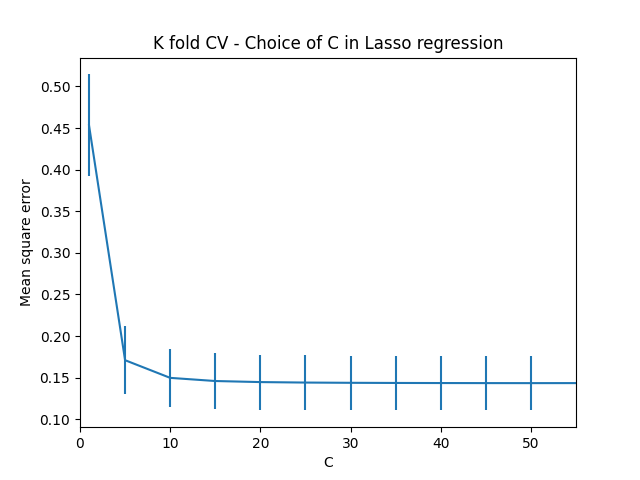
\includegraphics[scale=0.4]{Figure_4.png}
\end{center}
As we can observe from the confusion matrix and the accuracy, the Logistic Regression Model has an accuracy of 87.23{\%}.

\section*{Question b}
\textbf{Use sklearn to train linear SVM classifiers on your data (nb: be sure to use the
LinearSVC function in sklearn, not the SVC function).}
\subsection*{Part i}
\textbf{Train linear SVM classifiers for a wide range of values of the penalty parameter
C e.g. C = 0.001, C = 1, C = 100. Give the SVM model for predictions and
report the parameter values of each trained model.}
\vspace{5mm}

\vspace{1mm}

C = 0.001
\begin{equation*}
  \theta_{0} + \theta_{1}x_{1} + \theta_{2}x_{2} = 0.23620534 - 0.01144997x_{1} + 0.3997965x_{2}
\end{equation*}


C = 1
\begin{equation*}
  \theta_{0} + \theta_{1}x_{1} + \theta_{2}x_{2} = 0.64844145 - 0.09123326x_{1} + 1.77077696x_{2}
\end{equation*}
\vspace{1mm}

C = 100
\begin{equation*}
  \theta_{0} + \theta_{1}x_{1} + \theta_{2}x_{2} = 0.65660689 - 0.09287349x_{1} + 1.79129874x_{2}
\end{equation*}
\vspace{1mm}
For C=100, we had to increase the number of iterations for the values to converge.

\subsection*{Part ii}
\textbf{Use each of these trained classifiers to predict the target values in the training
data. Plot these predictions and the actual target values from the data, together
with the classifier decision boundary.}
\vspace{5mm}

C = 0.001
\begin{center}
  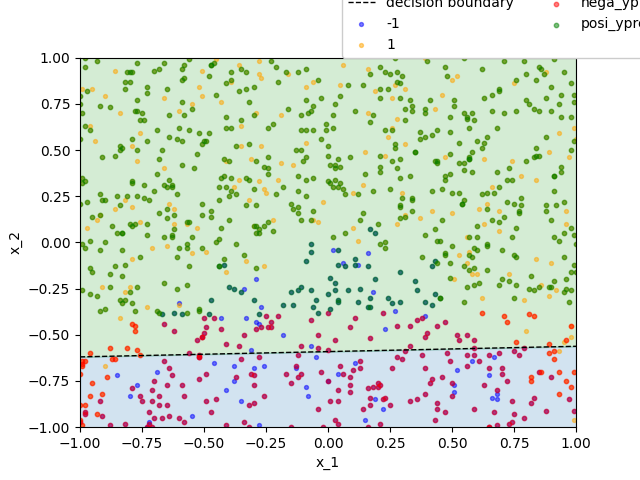
\includegraphics[scale=0.4]{Figure_5_001.png}
\end{center}
\vspace{5mm}

C = 1
\begin{center}
  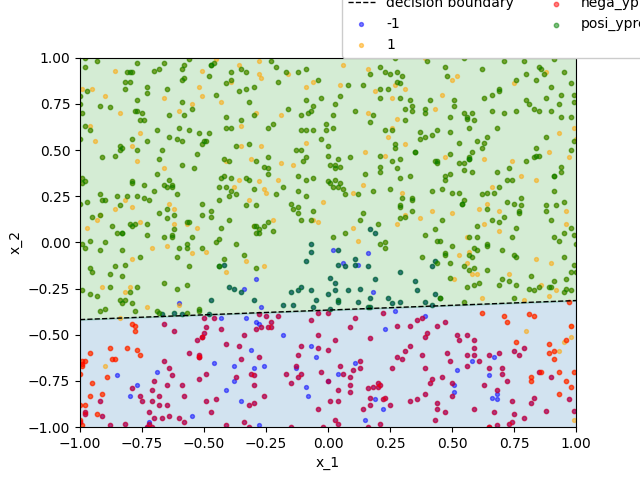
\includegraphics[scale=0.4]{Figure_5_1.png}
\end{center}
\vspace{5mm}

C = 100
\begin{center}
  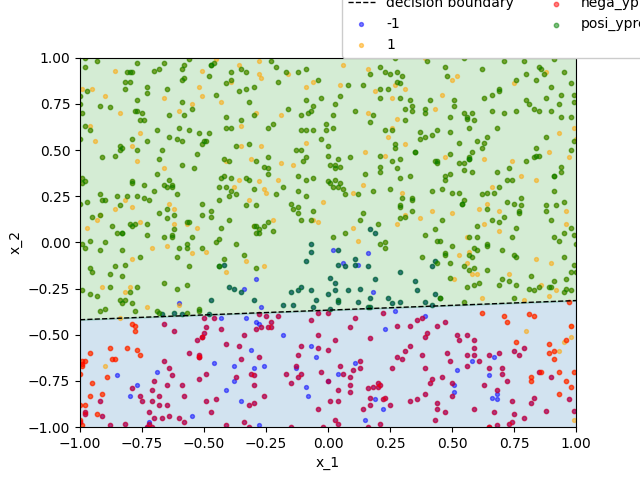
\includegraphics[scale=0.4]{Figure_5_100.png}
\end{center}
\vspace{5mm}

\subsection*{Part iii}
\textbf{What is the impact on the model parameters of changing C, and why? What
is the impact on the SVM predictions?}
\vspace{5mm}

As per definition, C is the penalty parameter of the error term. The trade off between a smooth decision boundary and classifying the training points correctly is controlled by the C value.
The C value is inversely proportional to the margin. Smaller margin means lower misclassification rate (i.e. the extent to which the model misqualifies data).

A point to note is that increasing the C value might lead to overfitting of the data.

We observe that as the C value increases, the misclassification rate decreases, thus improving the model's accuracy.
The Accuracy value for the three values of C are as follows:
\begin{center}
  \begin{tabular}{ |c | c | c | }
    \hline
    \textbf{C} & \textbf{Accuracy} \\ 
    \hline
    0.001 & 83.6\% \\  
    \hline
    1 & 87.35\% \\
    \hline
    100 & 87.35\% \\
    \hline
  \end{tabular}
\end{center}

\subsection*{Part iv}
\textbf{How do the SVM model parameters and predictions compare to those of the
logistic regression model in part (a)?}
\vspace{5mm}

The comparison of parameters for SVM Model and Logistic Regression are as follows:

\begin{center}
  \begin{tabular}{ |c|c | c | c | }
    \hline
    \textbf{Regression Model}&\textbf{Coefficients} & \textbf{Intercepts} & \textbf{Accuracy} \\ 
    \hline
    LogisticRegression & [-0.25638908,4.80424731] & 1.81954024 &  87.23\% \\
    \hline
    SVM(C=0.001)&[-0.01144997,0.3997965 ]& 0.23620534& 83.60\% \\
    \hline
    SVM(C=1)&[-0.09123326,1.77077696]&0.64844145 & 87.35\% \\
    \hline
    SVM(C=100)&[-0.09287349  1.79129874] & 0.65660689& 87.35\%\\
    \hline
  \end{tabular}
\end{center}

From the table above, we observe that for smaller value of C in SVM, the accuracy is almost 4\% lesser than Logistic Regression Model. For larger values of C in SVM, the accuracy is slightly better than the Logistic Regression Model \textendash 0.12\% which is almost negligible.

\section*{Question c}
\subsection*{Part i}
\textbf{Now create two additional features by adding the square of each feature (i.e.
giving four features in total). Train a logistic regression classifier. Give the
model and the trained parameter values.}
\vspace{1mm}
\begin{center}
\begin{equation*}
  \theta_{0} + \theta_{1}x_{1} + \theta_{2}x_{2} + \theta_{3}x_{3} + \theta_{4}x_{4} = 0.44446801 - 0.22742594x_{1} + 6.32595126x_{2} + 6.05620586x_{3} - 0.88229379x_{4}
\end{equation*}
\end{center}

The Confusion Matrix for the new data is as follows:
\begin{center}
  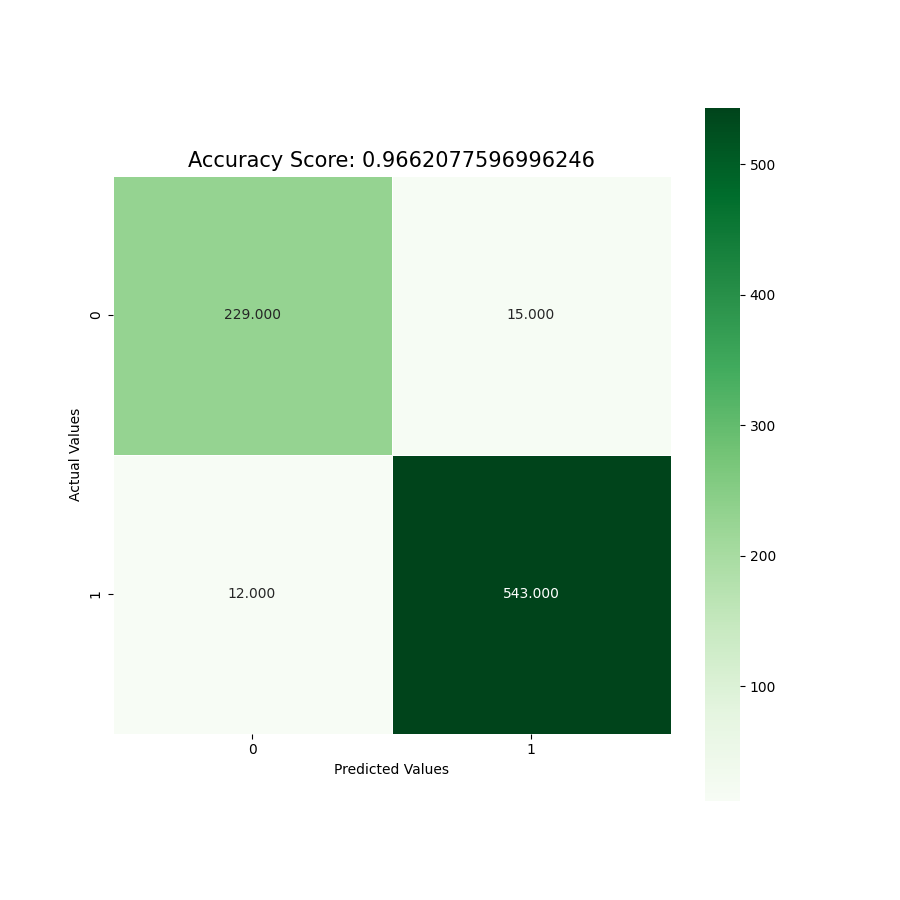
\includegraphics[scale=0.31]{Figure_6.png}
\end{center}


\subsection*{Part ii}
\textbf{Use the trained classifier to predict the target values in the training data. Plot
these predictions and the actual target values from the data using the same
style of plot as before i.e. using just the two original features as x and y axes.
Compare and discuss. How do the predictions compare with those in parts (a)
and (b) above?}

\begin{center}
  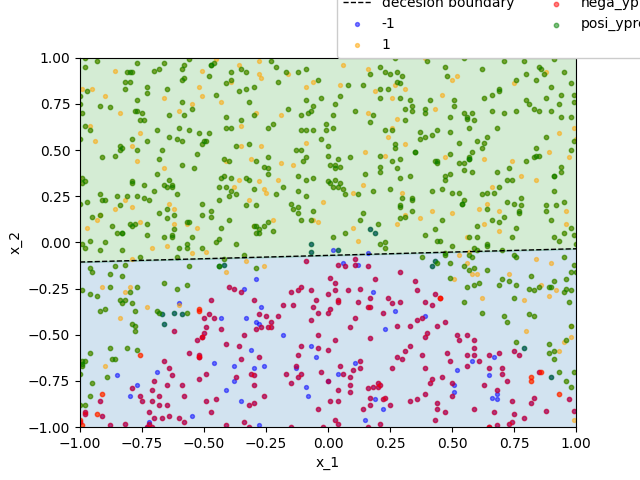
\includegraphics[scale=0.4]{Figure_7.png}
\end{center}

\subsection*{Part iii}
\textbf{Compare the performance of the classifier against a reasonable baseline predictor, e.g. one that always predicts the most common class.}
\vspace{1mm}

base model accuracy score:  0.7027027027027027 

trained model accuracy score:  0.9662077596996246

For my baseline predictor, I selected the mean classifier model.

Then I computed the accuracy against actual outputs for both the models: Logistic Regression Model and Baseline Model. We observe the following results:-


- Logistic Regression Classifier: 0.9662077596996246 (or 96.62\% accuracy)

- Baseline Model: 0.7027027027027027 (or 70.27\% accuracy)

Thus, we observe an increase of 26.35\% in the accuracy of our model which is a massive improvement.

\begin{center}
  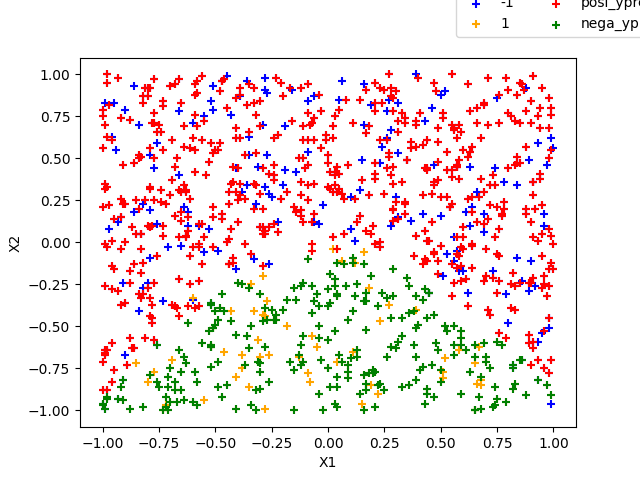
\includegraphics[scale=0.4]{Figure_8.png}
\end{center}

\section*{Appendix}
\textbf{Imports:}
\begin{lstlisting}[language=Python]
  import numpy as np
  import pandas as pd
  import matplotlib.pyplot as plt
  from sklearn.model_selection import train_test_split
  from sklearn.linear_model import LogisticRegression
  from sklearn.metrics import confusion_matrix
  import seaborn as sns
  from sklearn import metrics
  from sklearn.svm import LinearSVC
  from sklearn.model_selection import cross_val_score
  import statistics
\end{lstlisting}
\textbf{Question a i:}
\begin{lstlisting}[language=Python]
  plt.scatter(X1[y==1], X2[y==1], c='g', marker = '+', label='1')
  plt.scatter(X1[y==-1], X2[y==-1], c='b', marker = 'o', label='-1', s=10)
  plt.xlabel('x_1')
  plt.ylabel('x_2')
  plt.legend(bbox_to_anchor=(1.15,1.15), loc='upper right', 
  fancybox=True, framealpha=1, fontsize=10)
  plt.savefig('Figure_1.png')
\end{lstlisting}
\textbf{Question A ii and iii:}
\begin{lstlisting}[language=Python]
  LR=LogisticRegression()
  LR.fit(x_train, y_train)
  print('The slopes are: ',LR.coef_[0])
  print('The intercept is: ',LR.intercept_)
  predictions = LR.predict(x_train)
  score = LR.score(x_train, y_train)
  print('The score is: ',score)
  # FEATURE IMPORTANCE:
  feature_importance = LR.coef_[0]
  for i,val in enumerate(feature_importance):
    print('Feature: %0d, Score: %.5f' % (i,val))
  plt.bar([x for x in range(len(feature_importance))], feature_importance)
  plt.xlabel('Features')
  plt.ylabel('Scores')
  plt.savefig('Figure_2.png')
b_ = LR.intercept_[0]
w1, w2 = LR.coef_.T
c_ = -b_/w2
m_ = -w1/w2
x_min, x_max = -1, 1
y_min, y_max = -1, 1
x_d = np.array([x_min, x_max])
y_d = m_*x_d + c_
plt.plot(x_d, y_d, 'k', lw=1, ls='--',label='decision boundary')
plt.fill_between(x_d, y_d, y_min, color='tab:blue', alpha=0.2)
plt.fill_between(x_d, y_d, y_max, color='tab:green', alpha=0.2)
plt.scatter(*X[y==-1].T, s=10, alpha=0.5,label='-1',c='blue')
plt.scatter(*X[y==1].T, s=10, alpha=0.5,label='1',c='orange')
plt.scatter(*x_train[predictions==-1].T, s=10, alpha=0.5, 
label='nega_ypred',c='red')
plt.scatter(*x_train[predictions==1].T, s=10, alpha=0.5,
label='posi_ypred',c='green')
plt.xlim(x_min, x_max)
plt.ylim(y_min, y_max)
plt.ylabel('x_2')
plt.xlabel('x_1')
plt.legend(bbox_to_anchor=(1.2,1.2), loc='upper right', 
fancybox=True, framealpha=1,fontsize=10,ncol=2)
plt.savefig('Figure_3.png')
\end{lstlisting}
\textbf{Question b:}
\begin{lstlisting}[language=Python]
  lsvc001 = LinearSVC(C=0.001)
  print(lsvc001)
  lsvc001.fit(x_train, y_train)
  score = lsvc001.score(x_train, y_train)
  print("Score: ", score)
  cv_scores = cross_val_score(lsvc001, x_train, y_train, cv=10)
  print("CV average score: %.2f" % cv_scores.mean())
  print('The coefficients are: ',lsvc001.coef_[0])
  print('The intercept is: ',lsvc001.intercept_)
  lsvc1 = LinearSVC(C=1)
print(lsvc1)
lsvc1.fit(x_train, y_train)
score = lsvc1.score(x_train, y_train)
print("Score: ", score)
cv_scores = cross_val_score(lsvc1, x_train, y_train, cv=10)
print("CV average score: %.2f" % cv_scores.mean())
print('The coefficients are: ',lsvc1.coef_[0])
print('The intercept is: ',lsvc1.intercept_)
lsvc100 = LinearSVC(C=100,dual=False)
print(lsvc100)
lsvc100.fit(x_train, y_train)
score = lsvc100.score(x_train, y_train)
print("Score: ", score)
cv_scores = cross_val_score(lsvc100, x_train, y_train, cv=10)
print("CV average score: %.2f" % cv_scores.mean())
print('The coefficients are: ',lsvc100.coef_[0])
print('The intercept is: ',lsvc100.intercept_)
ypred001 = lsvc001.predict(x_train)
cm001 = confusion_matrix(y_train, ypred001)
print(cm001)
cr001 = metrics.classification_report(y_train, ypred001)
print(cr001)
bb = lsvc001.intercept_[0]
w1, w2 = lsvc001.coef_.T
cb = -bb/w2
mb = -w1/w2
xmin_b, xmax_b = -1, 1
ymin_b, ymax_b = -1, 1
xd_b = np.array([xmin_b, xmax_b])
yd_b = mb*xd_b + cb
plt.plot(xd_b, yd_b, 'k', lw=1, ls='--', label='decision boundary')
plt.fill_between(xd_b, yd_b, ymin_b, color='tab:blue', alpha=0.2)
plt.fill_between(xd_b, yd_b, ymax_b, color='tab:green', alpha=0.2)
plt.scatter(*X[y==-1].T, s=8, alpha=0.5,c='blue',label='-1')
plt.scatter(*X[y==1].T, s=8, alpha=0.5,c='orange',label='1')
plt.scatter(*x_train[predictions==-1].T, s=10, alpha=0.5, 
label='nega_ypred',c='red')
plt.scatter(*x_train[predictions==1].T, s=10, alpha=0.5,
label='posi_ypred',c='green')
plt.xlim(xmin_b, xmax_b)
plt.ylim(ymin_b, ymax_b)
plt.ylabel('x_2')
plt.xlabel('x_1')
plt.legend(bbox_to_anchor=(1.2,1.2), loc='upper right', 
fancybox=True, framealpha=1,fontsize=10,ncol=2)
plt.savefig('Figure_5_001')
ypred1 = lsvc1.predict(x_train)
cm1 = confusion_matrix(y_train, ypred1)
print(cm1)
cr1 = metrics.classification_report(y_train, ypred1)
print(cr1)
bb2 = lsvc1.intercept_[0]
w1, w2 = lsvc1.coef_.T
c_bb2 = -bb2/w2
m_bb2 = -w1/w2
xmin_bb2, xmax_bb2 = -1, 1
ymin_bb2, ymax_bb2 = -1, 1
xd_bb2 = np.array([xmin_bb2, xmax_bb2])
yd_bb2 = m_bb2*xd_bb2 + c_bb2
plt.plot(xd_bb2, yd_bb2, 'k', lw=1, ls='--',label='decision boundary')
plt.fill_between(xd_bb2, yd_bb2, ymin_bb2, color='tab:blue', alpha=0.2)
plt.fill_between(xd_bb2, yd_bb2, ymax_bb2, color='tab:green', alpha=0.2)
plt.scatter(*X[y==-1].T, s=8, alpha=0.5,c='blue',label='-1')
plt.scatter(*X[y==1].T, s=8, alpha=0.5,c='orange',label='1')
plt.scatter(*x_train[ypred1==-1].T, s=10, alpha=0.5, 
label='nega_ypred',c='red')
plt.scatter(*x_train[ypred1==1].T, s=10, alpha=0.5,
label='posi_ypred',c='green')
plt.xlim(xmin_bb2, xmax_bb2)
plt.ylim(ymin_bb2, ymax_bb2)
plt.ylabel('x_2')
plt.xlabel('x_1')
plt.legend(bbox_to_anchor=(1.2,1.2), loc='upper right', 
fancybox=True, framealpha=1,fontsize=10,ncol=2)
plt.savefig('Figure_5_1.png')
ypred100 = lsvc100.predict(x_train)
cm100 = confusion_matrix(y_train, ypred100)
print(cm100)
cr100 = metrics.classification_report(y_train, ypred100)
print(cr100)
bb3 = lsvc100.intercept_[0]
w1, w2 = lsvc100.coef_.T
c_b3 = -bb3/w2
m_b3 = -w1/w2
xmin_b3, xmax_b3 = -1, 1
ymin_b3, ymax_b3 = -1, 1
xd_b3 = np.array([xmin_b3, xmax_b3])
yd_b3 = m_b3*xd_b3 + c_b3
plt.plot(xd_b3, yd_b3, 'k', lw=1, ls='--',label='decision boundary')
plt.fill_between(xd_b3, yd_b3, ymin_b3, color='tab:blue', alpha=0.2)
plt.fill_between(xd_b3, yd_b3, ymax_b3, color='tab:green', alpha=0.2)
plt.scatter(*X[y==-1].T, s=8, alpha=0.5,c='blue',label='-1')
plt.scatter(*X[y==1].T, s=8, alpha=0.5,c='orange',label='1')
plt.scatter(*x_train[ypred100==-1].T, s=10, alpha=0.5, 
label='nega_ypred',c='red')
plt.scatter(*x_train[ypred100==1].T, s=10, alpha=0.5,
label='posi_ypred',c='green')
plt.xlim(xmin_b3, xmax_b3)
plt.ylim(ymin_b3, ymax_b3)
plt.ylabel('x_2')
plt.xlabel('x_1')
plt.legend(bbox_to_anchor=(1.2,1.2), loc='upper right', 
fancybox=True, framealpha=1,fontsize=10,ncol=2)
plt.savefig('Figure_5_100.png')
\end{lstlisting}
\textbf{Question c:}
\begin{lstlisting}
  LR1=LogisticRegression()
  LR1.fit(x_train1, y_train1)
  print('The Slopes are: ',LR1.coef_[0])
  print('The intercept is: ',LR1.intercept_)
  predictions1 = LR1.predict(x_train1)
  score1 = LR1.score(x_train1, y_train1)
  print('The score is: ',score1)
  XX=np.column_stack((X1**2,X2**2))
  bxx = LR1.intercept_[0]
  w=w1, w2, w3, w4 = LR1.coef_.T
  c_c = -bxx/w2
  m_c = -w1/w2
  xmin_c, xmax_c = -1, 1
  ymin_c, ymax_c = -1, 1
  xd_c = np.array([xmin_c, xmax_c])
  yd_c = m_c*xd_c + c_c
  plt.plot(xd_c, yd_c, 'k', lw=1, ls='--', label='decesion boundary')
  plt.fill_between(xd_c, yd_c, ymin_c, color='tab:blue', alpha=0.2)
  plt.fill_between(xd_c, yd_c, ymax_c, color='tab:green', alpha=0.2)
  plt.scatter(*X[y==-1].T, s=8, alpha=0.5,c='blue',label='-1')
  plt.scatter(*X[y==1].T, s=8, alpha=0.5,c='orange',label='1')
  plt.scatter(*x_train[predictions1==-1].T, s=10, alpha=0.5, 
  label='nega_ypred',c='red')
  plt.scatter(*x_train[predictions1==1].T, s=10, alpha=0.5,
  label='posi_ypred',c='green')
  plt.xlim(xmin_c, xmax_c)
  plt.ylim(ymin_c, ymax_c)
  plt.ylabel('x_2')
  plt.xlabel('x_1')
  plt.legend(bbox_to_anchor=(1.2,1.2), loc='upper right', 
  fancybox=True, framealpha=1,fontsize=10,ncol=2)
  plt.savefig('Figure_7.png')
  baseline_model = np.sign(statistics.mean(y))
ypred_baseline = np.full((len(y), 1), baseline_model)
LR_accuracy = metrics.accuracy_score(y_train1, predictions1)
baseline_accuracy = metrics.accuracy_score(y, ypred_baseline)
print("base model accuracy score: ", baseline_accuracy,
" - trained model accuracy score: ", LR_accuracy)
plt.scatter(X1[y==1], X2[y==1],color='blue', marker="+",label='-1')
plt.scatter(X1[y==-1], X2[y==-1],color='orange', marker="+",label='1')
plt.scatter(*x_train[predictions1==1].T,color='red', marker="+",
label='posi_ypred')
plt.scatter(*x_train[predictions1==-1].T,color='green', marker="+",
label='nega_ypred')
plt.xlabel("X1")
plt.ylabel("X2")
plt.legend(bbox_to_anchor=(1.2,1.2),loc='upper right',ncol=2,fontsize=10)
plt.savefig('Figure_8.png')
\end{lstlisting}
\end{document}